\newpage
\chapter{Accelerating Image Processing and SpMV}

\section{Basic Image Processing Application}

We need to compile vbxapi library present in MXP repository to use MXP API’s, on Linux. Once built, this library needs to be linked while compiling the application which we will write on Linux. To start with, we built application for image negation and scaling operations. The input and processed image obtained after running the image negation application are shown in Figure~\ref{lena:7}

\begin{figure}
	\centering
	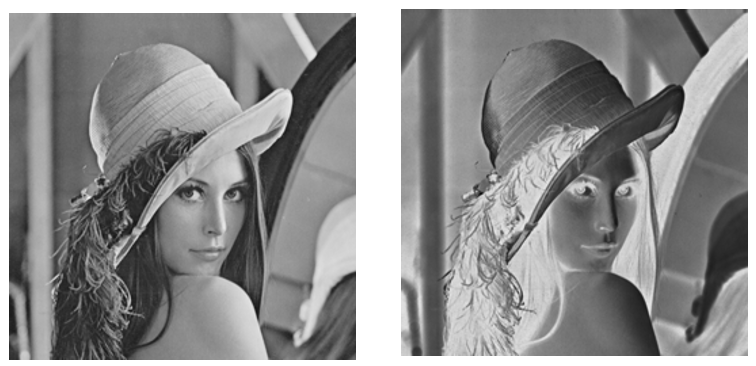
\includegraphics[width=.9\textwidth]{images/lena.png}
	\caption{Results of the Image Negation}
	\label{lena:7}
\end{figure}

The MXP application code for processing the input image for a negation operation is provided in Figure~\ref{cod:7}


%\lstinputlisting[firstline=89, lastline=132, frame=none,numbers=left,basicstyle=\fontsize{10}{10}\selectfont\ttfamily, backgroundcolor=\color{gainsboro}]{CodeSnippet.txt}


\begin{figure}
	\centering
	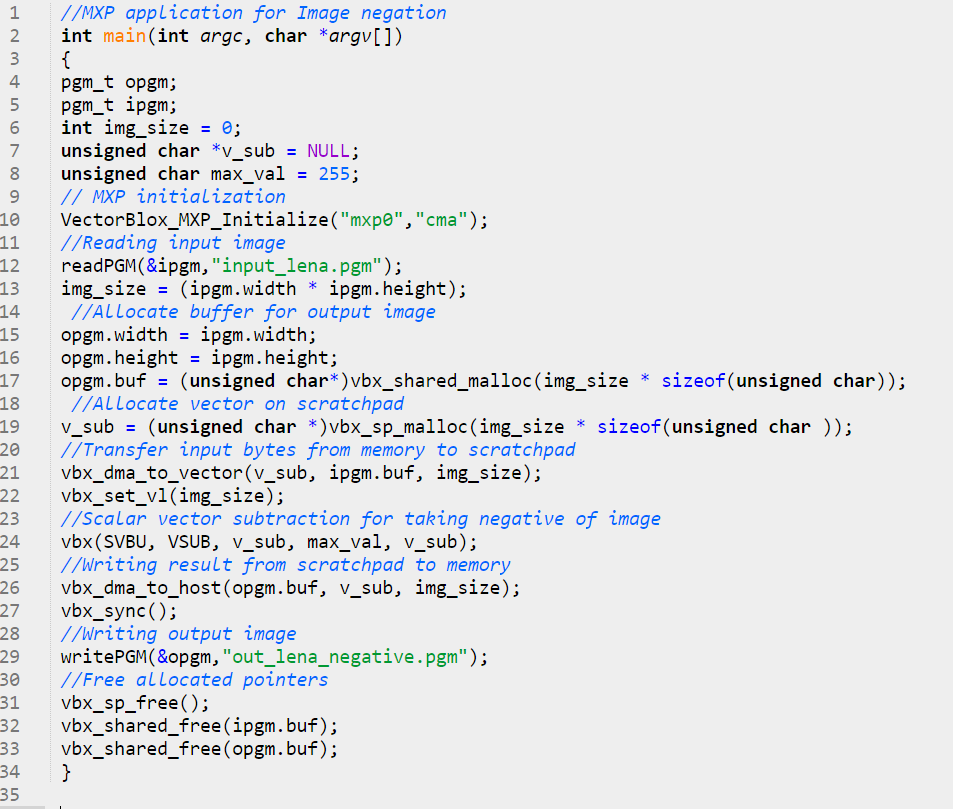
\includegraphics[width=1\textwidth]{images/code2.png}
	\caption{MXP application for Image negation}
	\label{cod:7}
\end{figure}


%\lstinputlisting[language=c,firstline=89, lastline=122, frame=none,numbers=left,basicstyle=\fontsize{11}{13}\selectfont\ttfamily, backgroundcolor=\color{gainsboro}]{hi.txt}

\section{Experiments and Results}

We took images of different dimensions and tried building image negative application for different platforms such as ARM v7, MXP and SIMD NEON unit. We tested the application with 128 X 128 pixels and 256 X 256 pixels. The runtime for the MXP soft-vector processor was then compared with the other processors. We observed that MXP seems to outperform other processors with a very good runtime obtained.  Table~\ref{ga:100} shows the runtime analysis of the MXP against the other processors.

\begin{table}[htbp]
	\centering
		\begin{adjustbox}{width=.9\textwidth}
		\small
	\begin{tabular}{lllll}
		\toprule
		\textbf{Metrics} & \textbf{ARMv7 CPU} & \textbf{NEON (auto vector)} & \textbf{MXP} \\
		\midrule
		\textbf{arch} & Scalar & SIMD unit & Vector \\
		\textbf{clock} & $667 x 10^{6}Hz$ & $667 x 10^{6}Hz$ & $110 x 10^{6}Hz$ \\
		\textbf{no of lanes} & 1 & 2 x 32b & 1-16 x 32b \\
		&   & 4 x 16b & 2-32 x 16b \\
		&   & 8 x 8b & 4-64 x 8b \\
		\midrule
	\textbf{Runtime (milliseconds)} &   &   &  \\
		\midrule
     128 x  128      pixels & 0.406 & 0.424 & 0.03686  \\	
	 256 x  256      pixels & 1.714 & 1.198 & 0.1843  \\
		\bottomrule
	\end{tabular}%
     \end{adjustbox}%
	\caption{Image Processing Runtime Analysis}
		\label{ga:100}%
\end{table}%



\section{Accelerating the SpMV Computational Kernel}

Sparse matrix dense vector also known as SpMV is one of the widely used computational kernel. It finds its application to solve the sparse linear system in information retrieval and many other applications. Since it is widely used, it is important to have a benchmark for SpMV. However, SpMV is really very difficult to benchmark because the data structure which is used in sparse matrix, it's density of the non-zero entries and it's dimensions - all have a significant impact on SpMV performance \cite{24},\cite{25}. We present a method on how the pre-existing benchmark for SpMV can be used and how MXP soft-processor can be used to accelerate the SpMV.

\subsection{SpMV basics}
	
In the case of a dense matrix, simple contiguous array is used as the data structure containing all the entries. Two orderings are most common: 
\begin{enumerate}

	\item row- major, where the rows are stored contiguously.
	\item column-major, where the columns are stored contiguously.
 
\end{enumerate}

The sparse multiplication depends on the structure of the sparse matrix. We can have regular and irregular structure for the SpMV. The general idea of performing a SpMV is to decompose the matrix into regular and the irregular parts. Compressed Sparse Row Format and Compressed Sparse Column Format are the basic formats in which the sparse matrix 
are stored.

\subsubsection{Compressed Sparse Row Format}

In CSR format, all the nonzero entries of the matrix will be in the form of row-major order consisting of two different arrays namely row\_start and col\_idx. The row\_start consist of index of non-zero entry present in the matrix in each row and the col\_index consist of the index of the non-zero entry present in the matrix in each column. Figure~\ref{aa:100} shows how the matrix elements will be stored while using the CSR format.

\begin{figure}
	\centering
	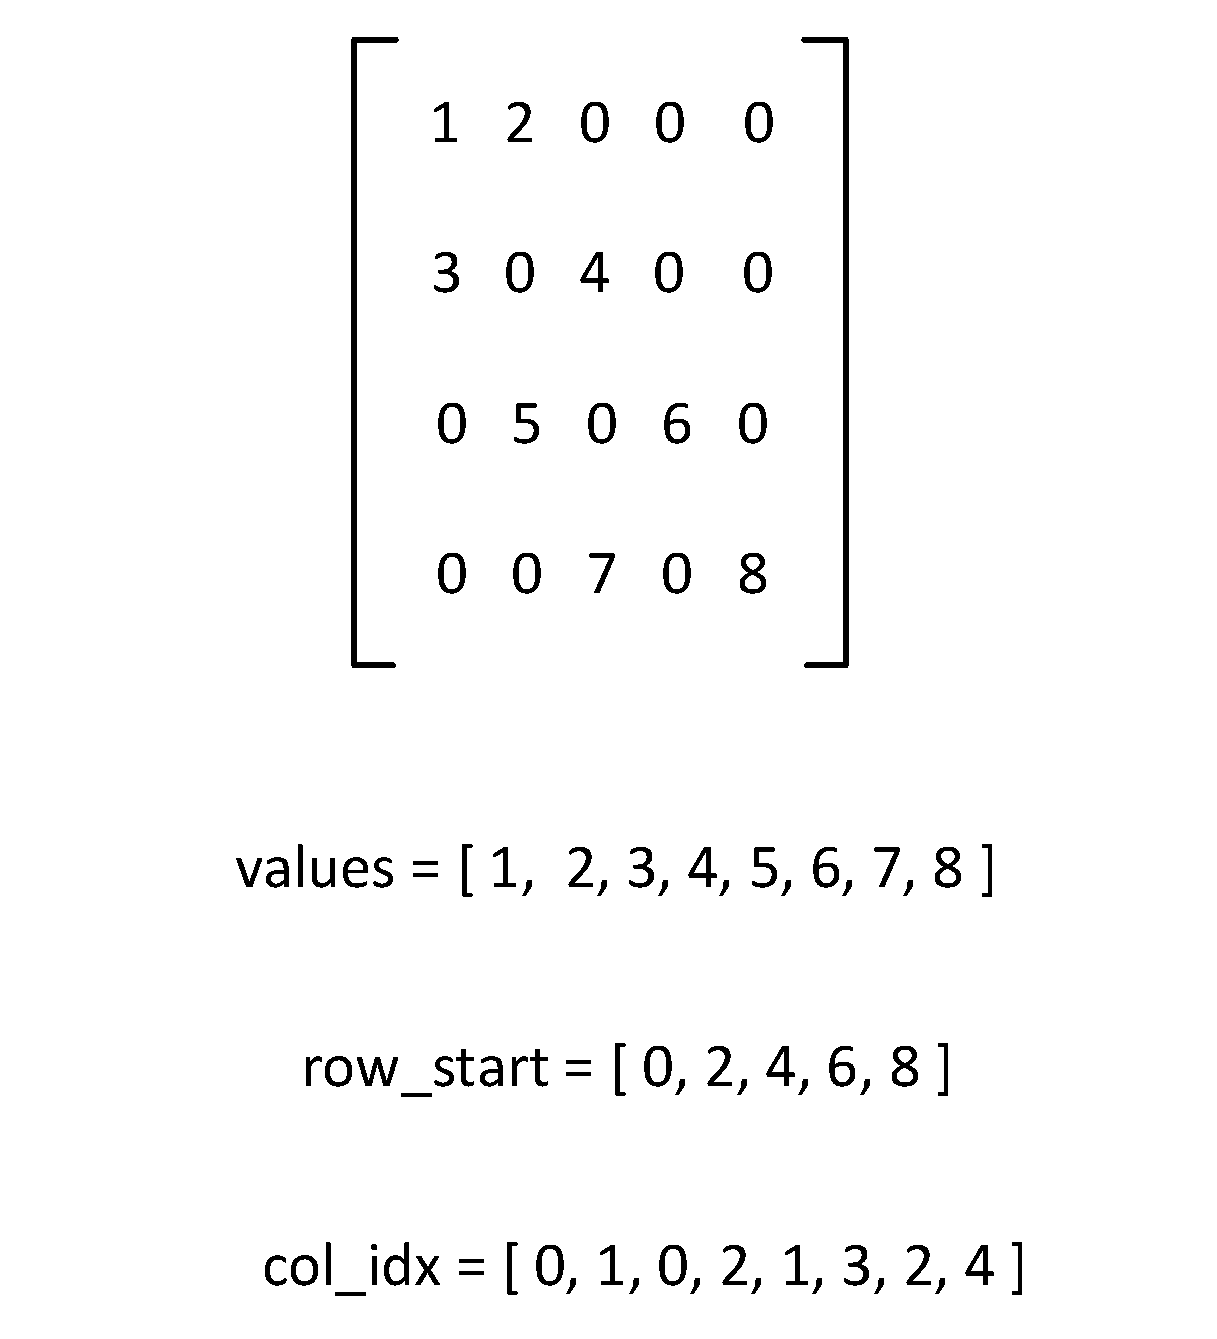
\includegraphics[width=.4\textwidth]{images/csr.pdf}
	\caption{Compressed Sparse Row Format}
	\label{aa:100}
\end{figure}

\subsubsection{Compressed Sparse Column Format}

In CSC format, all the nonzero entries of the matrix are kept in form of column major order consist-ing of two arrays namely col\_start and row\_idx. The col\_index consists of index of element of each row present and row\_idx consist of the index of the non-zero entry present in each row of matrix. The figure shows how the matrix elements will be stored while using the CSR format. When above Figure~\ref{aaa:1000} is stored in Compressed Sparse Row (CSR), it will be represented in the following form

\begin{figure}
	\centering
	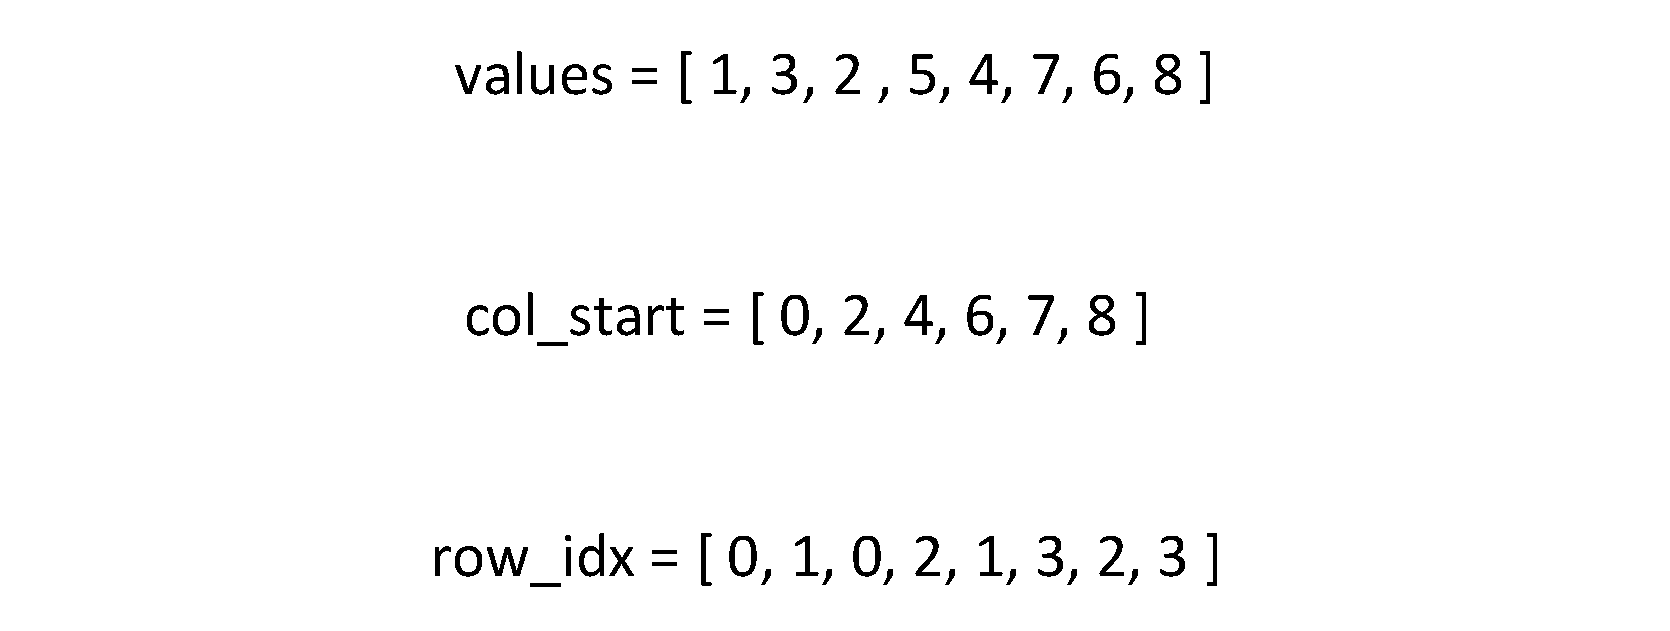
\includegraphics[width=.6\textwidth]{images/csc.pdf}
	\caption{Compressed Sparse Column Format}
	\label{aaa:1000}
\end{figure}

\subsection{Details of Pre-existing SpMV Benchmark}

The Pre-existing benchmarking framework mentioned in \cite{24}, stores the elements of the matrix in BCSR (Blocked Compressed Sparse Row) format. The idea behind the BCSR is to divide a given sparse matrix of size m x n into blocks of size r x c. By doing so we would obtain m / r blocks of rows and n / c blocks of columns which further can be stored in CSR format. Hence, at the end we will obtain m / r blocks where each of them represents r number of rows of the matrix and n / c blocks where each of them represents c number of columns of the matrix. This method helps in improving the accessing the elements of the sparse matrix and efficiently storing them in contiguous array either in row order or column order form. The operations are performed very efficiently providing high speedups. The blocks inside the dense matrix in Figure~\ref{aaaa:10000} are coloured and row major ordering is being used.  


\begin{figure}
	\centering
	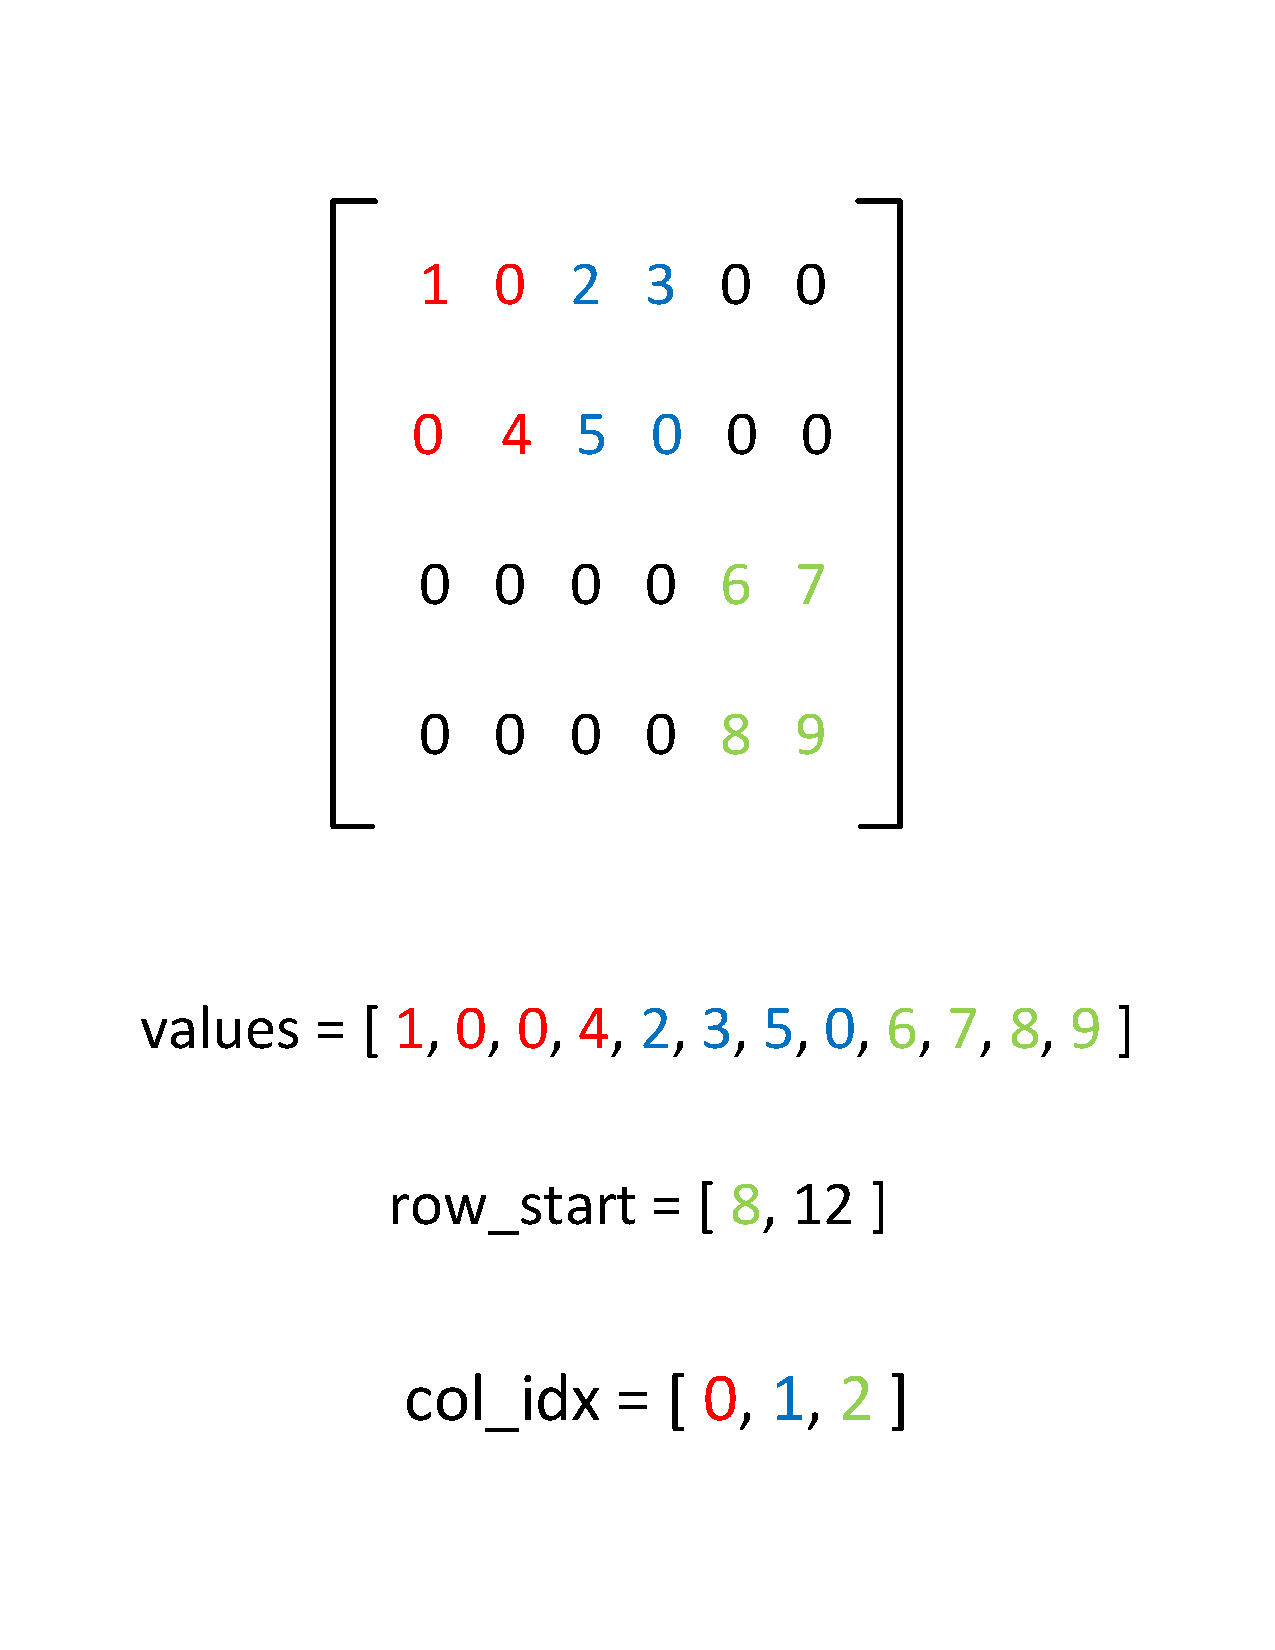
\includegraphics[width=.6\textwidth]{images/bcr.pdf}
	\caption{Blocked Compressed Sparse Row ordered}
	\label{aaaa:10000}
\end{figure}

\subsection{SpMV Usage Parameters}

When the main application will run in the existing framework it will generate the following usage parameters. User have the freedom to select one of the pre-defined block size. Below are the results which were obtained when Block Dim (r x c) was by default set to 1 x 1. Table~\ref{ww:101} shows the list of the SpMV usage parameters.
%\begin{figure}
%	\centering
%	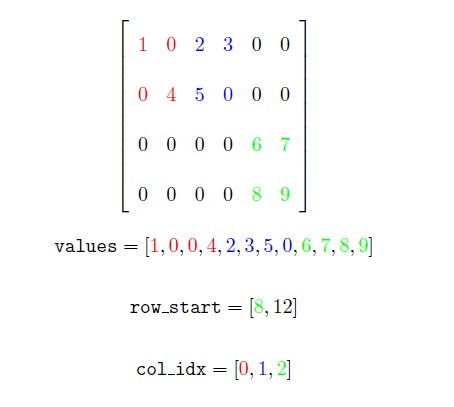
\includegraphics[width=.6\textwidth]{images/bcsr.jpg}
%	\caption{Blocked Compressed Sparse Row ordered}
%	\label{aaaa:10000}
%\end{figure}



\begin{table}[htbp]
	\centering	
	\begin{adjustbox}{width=.4\textwidth}
		\small
  \begin{tabular}{ll}
		\toprule
		\textbf{Parameters} & \textbf{Usage} \\
		\midrule
		   SpMV time & 0.886775 \\
		   Oper Time & 0.886774 \\
		   Cache time & 0.000001 \\
		   Matrix Dim (r x c) & 2097152 x 2097152 \\
		   Block Dim (r x c) & 1 x 1 \\
		   Non-zero blocks & 71303168 \\
		   Repetitions & 1 \\
		   Mflop/s & 160.814565 \\
		   num\_loads & 293601308 \\
		   num\_stores & 570425344 \\
		\bottomrule
	\end{tabular}%
\end{adjustbox}%
\caption{SpMV Usage}
\label{ww:101}%
\end{table}%

This pre-existing benchmarking framework consist of the block routine of dimensions \{2 x 2\}, \{4 x 4\}, \{8 x 8\}... Based on the block size we divide the sparse matrix into different blocks. This gives some hint to accelerate this benchmarking framework for SpMV by changing these block routines using the MXP APIs.


\subsection{Accelerating SpMV Framework Using MXP APIs}

MXP APIs are configured for the existing benchmarking framework so that we can use these APIs to accelerate the benchmarking process of the SpMV. There are block routines which are present in the existing framework. These block routines operate on the given sparse matrix at the block level. Thus, using the MXP APIs the block routines are modified to improve its performance.  Table~\ref{www:1010} shows the speedup obtained while performing SpMV multiplication which is in the form of $y = Ax$, one of the widely used computational kernel where A is a Sparse Matrix and x is the input vector and output y is the dense matrix.


\begin{table}[htbp]
	\centering
	
	\begin{adjustbox}{width=.7\textwidth}
		\small
		
	\begin{tabular}{lllll}
		\toprule
		\textbf{Metrics} & \textbf{ARMv7 CPU} & \textbf{MXP}  \\
		\midrule
		\textbf{uarch} & Scalar & Vector \\
		\textbf{Clock} & $667 X 10^{6} Hz$ & $110 X 10^{6}Hz$  \\
		\textbf{No of Lanes} & 1 & 1-16 x 32b  \\
		&   & 2-32 X16b  \\
		&   & 4-64 X8b \\
		&   &   \\
		\midrule
		\textbf{Runtime (millisecond)  } &   &   &   &  \\
		\midrule
		\textbf{SpMV \{25 x 25\} kernel} & 0.037 & 0.01843  \\
		\textbf{SpMV \{50 x 25\} kernel} & 0.055 & 0.03686  \\
		\bottomrule
	\end{tabular}%
    \end{adjustbox}%
      \caption{Runtime for SpMV kernel Computation}
	\label{www:1010}%
\end{table}%	
    	 

\section{SpMV Kernel Code}

The algorithm along with the code for calculating the runtime for SpMV kernel Computation can be found in the below link:

Github Link : \url{https://github.com/AdhikariSaurabh/mxpbenchmarks/tree/master/SpMV}






